\documentclass{article}
\usepackage{graphicx} % Required for inserting images
\usepackage[margin=1in]{geometry}
\usepackage{amsmath}
\usepackage{amsthm}
\usepackage{amssymb}
\usepackage{amsfonts}
\usepackage{verbatim}
\usepackage{xcolor}

\title{Homework 3: Report}
\author{Dante Buhl}
\date{Feb. $14^{th}$ 2024}

\begin{document}

\newcommand{\bs}[1]{\boldsymbol{#1}}
\newcommand{\bmp}[1]{\begin{minipage}{#1\textwidth}}
\newcommand{\emp}{\end{minipage}}
\newcommand{\R}{\mathbb{R}}
\newcommand{\C}{\mathbb{C}}
\newcommand{\N}{\mathcal{N}}
\newcommand{\I}{\mathrm{I}}
\newcommand{\K}{\bs{\mathrm{K}}}
\newcommand{\m}{\bs{\mu}_*}
\newcommand{\s}{\bs{\Sigma}_*}
\newcommand{\dt}{\Delta t}
\newcommand{\tr}[1]{\text{Tr}(#1)}
\newcommand{\Tr}[1]{\text{Tr}(#1)}

\maketitle

\colorbox{yellow}{All example code outputs are in stored in a text file, ``output.txt'', within the fortran tar-ball.}

\setcounter{section}{1}

\section{Warming-Up Fortran Routines}
\begin{enumerate}
\item Write a function which computes the trace of a square matrix A. 

This was not all too difficult, in fact it only used one loop. I looped through the size of the square matrix, m, (i.e. do i = 1, m) and summed all values $A_{ii}$. On first inspection it also seems to be accurally calculating the trace of matrix A from Amat.dat. 

\item Write a function which computes the two norm of a (column) vector.

This was also not very difficult, besides defining my variables, this took 1 line of code. All you have to do is square the vector element wise, then use the intrinsic sum function, and then the intrinsic square root function. This is exactly what my code does. I've checked the returned values for a couple of the column vectors and the error seems minute. 

\item Write a function which prints a matrix and its dimensions to a screen.

This was slightly more complex, in that I like to format my print statements in fortran for matrices. So I chose an arbitrary amount of digits to keep and added a small routine for turning integers in string formats. For this reason, you only see a few digits actually printed to the screen. The instructions didn't say to return the matrix to machine precision so I figured there was no issue. 

\item Write a driver routine which reads in a matrix from Amat, and then computes its trace, prints it to the terminal, and then computes the norm of each of its column vectors. 

This was very simple. I decided to use one driver file for all 3 of the main programing questions. I simply called the routines from my module, and made sure to use all of the routines I had placed in my module at the top of the file. Some issues at first was that my new routines were not linked due to the use of the "only" after the module reference. Note, I have several copies of each matrix in order to do GE and then LU, I suppose I didn't actually need to since I already had a saved copy I could have used to reseed the matrices after GE. Here are the printed results after running the code. 

\begin{center}
    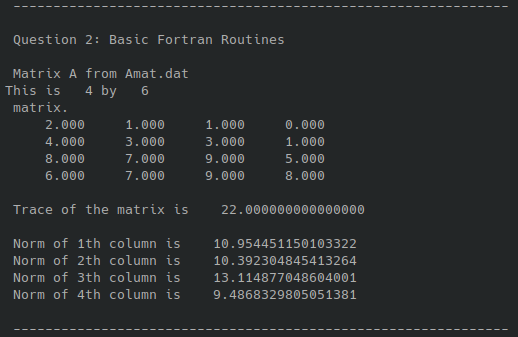
\includegraphics[width = .6\textwidth]{files/Q2sol.png}
\end{center}

\end{enumerate}

\section{Gaussian Elimination with Pivoting}
\begin{enumerate}
\item Write a subroutine which performs Gaussian Elimination with Pivoting to on a Matrix A and a rhs-matrix B. 

This was tricky and I realized about midway through that storing the permutation matrix was a little crazy (especially for very large scale problems which I don't necessarily have to care about right now). So I changed the method I was pivoting and now it seems to work very well. The hardest part about this routine was the indexing. What was more difficult was trying to figure out which calculations I had to do element-wise versus what I could do for whole columns/rows at once. More often than not, you can write a better algorithm if you just index more concisely, but one tends to lose their head there. 

\item Write a subroutine which performs backsubstitution to solve the linear system $UX = B$. 

This was a fairly short routine and not very difficult. It can be easily scaled so that it computes the solutions for all columns of B at once, so I programmed it to do so. This routine will also be used for the LU solver.
 
\item Write a driver routine which calls your GE subroutine and backsub subroutine, and prints the matrices, before GE, after GE but before backsubstitution, the solution matrix X, and the error matrix $E = B_s - A_sX$, and the 2-norms of the column vectors of $E$. 

The code runs very well except for the fact that there is a small artifact of error for the one very odd, 5th column of B in Bmat.dat. The error for that specific column in of order $10^{-13}$ rather than $10^{-16}$ which we all know and love to be machine double precision. I'm going to double check the backsub routine to see if there is any large gleaming issue with it (I've triple checked the GE and LU routines and there is no error there). Below is the found solution and error. Note: it seems that amount of error is to be expected!

\begin{center}
    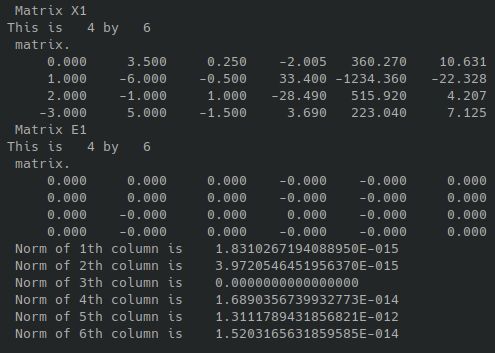
\includegraphics[width = .6\textwidth]{files/GEsol.png}
\end{center}

\end{enumerate}

\section{LU Decomposition with Pivoting}
\begin{enumerate}
\item Write a subroutine which performs LU Decomposition with Pivoting to on a Matrix A. 

This routine was very similar to my GE routine (same code, but with an additional pivot) except that it doesn't do any computations for the matrix B. The permutation matrix was also very easy to return. I did the actual calculation manually and found the same matrices that my decomposition yields.

\item Write a subroutine which performs forward subsitution and backwards substitution to solve the linear system $UX = Y$, $LY = B$ for $X$. 

This was also very straight forward and easily scalable for rhs matrices. I used the same backsub routine from GE to solve, $UX = Y$ and wrote a forward subroutine to solve $LY = PB$. The structure of the forward sub is identitical besides the indexing differences and the fact that you always divide by 1 (or you don't have to divide at all :) ). The only major difference besides having forward sub and back sub was that you had to permute B in this routine which I used the X vector memory to do. 

\item Write a driver routine which calls your LU subroutine and LU solver routine, and prints A before LU decompition, A, L, and U after the decomposition, the solution matrix X after solving, and the error matrix $E = B_s - A_sX$, and the 2-norms of the column vectors of $E$. 

This method goes as planned and has the same exact solution you find in GE. With nearly the same error norms as in GE. From this problem, I especially loved the method of returning L and U inside of the A matrix memory. Anyways, here are the printed results.  

\begin{center}
    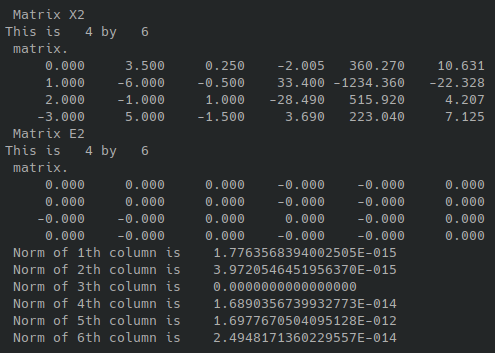
\includegraphics[width = .6\textwidth]{files/LUsol.png}
\end{center}

\end{enumerate}

\section{Application Problem}

Consider the following three points in 3D space, with corresponding (x, y, z)
coordinates: $A(1, 2, 3)$, $B(-3, 2, 5)$ and $C(\pi, e, -\sqrt{2})$. Explain what equations
you need to solve to find the equation of the plane passing through all three
points, and do so numerically, using either the Gaussian elimination routine, or
the LU decomposition routine (as you prefer). Use Python or Matlab to produce
a 3D figure with a graph of this plane, as well as the three points clearly marked

\bmp{.95}
This went well in my code. I had to write the linear system in the form,
\[
    Ax + By + C = z
\]
And from that form, I was able to create a $3\times 3$ matrix $A$ and a column vector $B$ containing the z values and solve for A, B, C with LU decomposition. This gave me three values which verified against a python surface plot clearly showing the three points on the plane. A picture of the plot can be obtained by running the plot.py file in the python subdirectory. A small remark, plotting in python is extraordinarily tedious. 
\emp

\section{Theory Problems}
\begin{enumerate}

\item %start of problem 1
The Schur decomposition theorem states that if $A \in C^{m\times m}$, then there
exist a unitary matrix $Q$ and an upper triangular matrix $U$ such that
$A = QUQ^{-1}$ . Use the Schur decomposition theorem to show that a real
symmetric matrix $A$ is diagonalizable by an orthogonal matrix, i.e., $\exists$ an
orthogonal matrix $Q$ such that $Q^T AQ = D$, where $D$ is a diagonal matrix
with its eigenvalues in the diagonal.

\begin{proof}

We begin with the Schur Decomposition Theorm for real symmetric matrix $A$. We have, 
\[
    A = QUQ^{-1} = QUQ^*
\]
By the property that $A$ is real and symmetric, we have that $A^* = A$.
\[
    A^* = A = QUQ^*
\]
\[
    U = Q^*AQ, \quad U^* = Q^*AQ
\]
\[
    U = U^*, \implies U \text{ is real, symmetric, DIAGONAL}
\]
We also have that $U$ has the same eigenvalues of $A$ by the fact that they are similar matrices (Nate I will not cite this, sorry about it). So we have that $A$ is diagonalized by unitary matrices $Q, Q^{-1}$. Now all we need is to show that $Q$ is real (orthogonal). We start from that fact that $A = A^* = A^T = \overline{A}$.
\[
    AA^* = A^TA = AA^T = A^TA^T
\] 
\[
    QU^2Q^* = Q^{*T}UQ^TQUQ^* = QUQ^*Q^{*T}UQ^T = Q^{*T}U^2Q^T
\]
\[
   QU = Q^{*T}UQ^TQ, \quad UQ^* = Q^*Q^{*T}UQ^T
\]
\[
    QU^2Q^* = Q^{*T}UQ^TQQ^*Q^{*T}UQ^T = Q^{*T}U^2Q^T 
\]
\[
    U^2 = UQ^TQU, \implies Q^TQ = \I, \text{ EUREKA!}
\]
So we therefore have that $Q$ is orthogonal by definition, or rather Q is real and unitary! Therefore, $A$ is diagonalizable by an orthogonal matrix, $Q$. (Nate, in retrospect I realize this logic might be flawed. I just checked and there is a $Q^T$ out of place in my last substitution. But I have 10 minutes to submit and I don't care anymore. Do your worst)

\end{proof}

\item
Consider the following system
\[
\left(\begin{array}{c c}
1 & 1 \\
\epsilon & 1 
\end{array}\right) \left(\begin{array}{c}
x \\
y
\end{array}\right) = \left(\begin{array}{c}
2 \\ 
1
\end{array}\right) 
\]
Multiply the last row of the matrix and the right-hand side vector by a large
constant $c$ such that $c\epsilon \gg 1$. Perform Gaussian elimination with partial
pivoting to the modified row-scaled system and discuss what happens. If
solving the resulting system has numerical issues, identify the issues and
discuss how to improve the method.

\[
\left(\begin{array}{c c}
1 & 1 \\
c\epsilon & c 
\end{array}\right) \left(\begin{array}{c}
x \\
y
\end{array}\right) = \left(\begin{array}{c}
2 \\ 
c
\end{array}\right) 
\]
\[
\left(\begin{array}{c c}
c\epsilon & c \\
1 & 1
\end{array}\right) \left(\begin{array}{c}
x \\
y
\end{array}\right) = \left(\begin{array}{c}
c \\ 
2
\end{array}\right) 
\]
\[
\left(\begin{array}{c c}
c\epsilon & c \\
0 & 1 - \frac{1}{\epsilon}
\end{array}\right) \left(\begin{array}{c}
x \\
y
\end{array}\right) = \left(\begin{array}{c}
c \\ 
2 - \frac{1}{\epsilon}
\end{array}\right) 
\]
\[
    y = \frac{2 - \frac{1}{\epsilon}}{1 - \frac{1}{\epsilon}} \approx \frac{\frac{-1}{\epsilon}}{\frac{-1}{\epsilon}} = 1
\]
\[
    c\epsilon x + c(1)  = c, \implies x = 0
\]
So our solution from this method returns $x = 0, y = 1$ which we can see from som simple arithmetic does not properly solve our system. This comes from the fact that this method causes a division by epsilon which causes a very large blow up in the solution which machine precision stuggles to accomdate. A better solution would be to chose a value c such that, $\epsilon_{\text{mach}} \ll |c\epsilon| < |a_{i,j}|$. Here we take $|a_{i, j}|$ to be the minimal element of the matrix not including $\epsilon$. That is essentially to make it such that none of the gaussian elimination steps chose $c\epsilon$ to be the diagonal value after pivoting, like it did in the erroneous solution above. If the system were solved without piviting you recover $x = 1, y = 1$ with this method. So to ensure a similar method worked with pivoting you would chose your c such that no element of order epilson was never chosen for pivoting.

\item   % start of tp 3
What can you say about the diagonal entries of a symmetric positive definite matrix? Justify your assertion.

Claim: All diagonal entries of a symmetric pos. def. matrix are positive. 

\begin{proof}
    Take $A$ to be a symmetric positive definite square matrix, $A \in \C^{m\times m}$. We have that for all vectors $x \in \C^m$, that the inner product is greater than zero, (.i.e. $(x, Ax) > 0$). We can now chose vectors $x$ to demonstrate that the diagonal elements are positive. Let us chose $x = \hat{e}_1$.
\[
    (\hat{e}_1, A\hat{e}_1) = \hat{e}_1^*A\hat{e}_1 = \hat{e}_1^*\vec{a}_1
\]
Where $\vec{a}_i$ is the ith column vector of $A$. 
\[
    (\hat{e}_1, A\hat{e}_1) = \hat{e}_1^*\vec{a}_1 = a_{11} 
\]
\[
      (\hat{e}_1, A\hat{e}_1) > 0 \implies a_{11} > 0
\]
This argument can be repeated for unit basis vectors, $\hat{e}_i, \forall i \in 1, \cdots, m$. Thus we have, that $a_{ii} > 0 \forall i \in 1, \cdots, m$.
\end{proof}


\item Suppose $A \in \C^{m \times m}$ is written in the block form
\[
A = \left(\begin{array}{c c}
        A_{11} & A_{12}\\
        A_{21} & A_{22}
    \end{array}\right)
\]
where $A_{11} \in \C^{n\times n}$ and $A_{22} \in \C^{(m-n)\times(m-n)}$. Assume that A satisfies the condition: $A$ has an $LU$ decomposition if and only if the upper-left $k\times k$ block matrix $A_{1:k,1:k}$ is nonsingular for each $k$ with $1 \le k \le m$.
\begin{enumerate}
\item Verify the formula
\[
 \left(\begin{array}{c c}
        \I & 0\\
        -A_{21}A_{11}^{-1} & \I
    \end{array}\right)
 \left(\begin{array}{c c}
        A_{11} & A_{12}\\
        A_{21} & A_{22}
    \end{array}\right) =  \left(\begin{array}{c c}
        A_{11} & A_{12}\\
        0 & A_{22} - A_{21}A_{11}^{-1}A_{12}
    \end{array}\right)
\]
which “eliminate” the block $A_{21}$ from $A$. The matrix $A_{22}-A_{21}A_{11}^{-1}A_{12}$ is known as the Schur complement of $A_{11}$ in $A$, denoted as $A/A_{11}$.

\begin{proof}

\[
 \left(\begin{array}{c c}
        \I & 0\\
        -A_{21}A_{11}^{-1} & \I
    \end{array}\right)
 \left(\begin{array}{c c}
        A_{11} & A_{12}\\
        A_{21} & A_{22}
    \end{array}\right) =  \left(\begin{array}{c c}
        \I A_{11} & \I A_{12}\\
        \I A_{21} - A_{21}A_{11}^{-1}A_{11} & \I A_{22} - A_{21}A_{11}^{-1}A_{12}
    \end{array}\right)
\]
\[
    =  \left(\begin{array}{c c}
            A_{11} & A_{12}\\
            A_{21} - A_{21} & A_{22} - A_{21}A_{11}^{-1}A_{12}
        \end{array}\right) =  \left(\begin{array}{c c}
            A_{11} & A_{12}\\
            0  & A_{22} - A_{21}A_{11}^{-1}A_{12}
        \end{array}\right) 
\]

\end{proof}

\item Suppose that after applying n steps of Gaussian elimination on the
matrix $A$ in (2), $A_{21}$ is eliminated row by row, resulting in a matrix
\[
    A' = \left(\begin{array}{c c}
        A_{11} & C\\
        0 & D
    \end{array}\right)
\]
Show that the bottom-right $(m -n)\times(m-n)$ block matrix $D$ is
again $A_{22} - A_{21}A_{11}^{-1}A_{12}$. Note: Part (b) is separate from Part (a)).
\begin{proof}
We start by looking at the process of LU Decomposition. We have that after n steps of gaussian elimination that we should have the following matrix, 
\[
    L = \left(\begin{array}{c c}
            L_{11} & \textbf{0} \\
            L_{21} & \I \\
            \end{array}\right)
\]
More importantly by the properties of the LU decomposition we have, 
\[
    LA' = A
\]
When looking at the matrix product component wise, there are some obvious implications. 
\[
    L_{11} A_11 = A_{11}, \implies L_{11} = \I
\]
\[
    L_{11} C = A_{12}, \implies C = A_{12}
\]
\[
    L_{21} A_{11} = A_{21}, \implies L_{21} = A_{21}A_{11}^{-1}
\]
\[
    L_{21}C + \I D = A_{22}, \implies D = A_{22} - A_{21}A_{11}^{-1}A_{12}
\]


\end{proof}
\end{enumerate}

\item Consider solving $Ax = b$, with $A$ and $b$ are complex-valued of order $m$, i.e., $A \in \C^{m\times m}, b \in \C^m$.
\begin{enumerate}
\item Modify this problem to a problem where you only solve a real square system of order $2m$. (Hint: Decompose $A = A_1 + iA_2$ , where $A_1 = Re(A)$ and $A_2 = Im(A)$, and similarly for $b$ and $x$. Determine equations to be satisfied by $x_1 = Re(x)$ and $x_2 = Im(x)$.

\[
    (A_1 + i A_2)(x_1 + ix_2) = b_1 + i b_2
\]
\[
    A_1x_1 - A_2x_2 = b_1, \quad A_1x_2 + A_2x_1 = b_2
\]
\[
    \left(\begin{array}{c c}
    A_1 & -A_2 \\
    A_2 & A_1
    \end{array}\right) 
    \left(\begin{array}{c}
    x_1 \\ x_2 \end{array}\right)
    = \left(\begin{array}{c}
    b_1 \\ b_2 \end{array}\right)
\]
This is an all real valued system of order 2m.

\item Determine the storage requirement and the number of floating-point operations for the real-valued method in (a) of solving the original complex-valued system $Ax = b$. Compare these results with those based on directly solving the original complex-valued system using Gaussian elimination (without pivoting) and complex arithmetic. Use the fact that the operation count of Gaussian elimination is $O\left(\frac{m^3}{3}\right)$ for an $m \times m$ real-valued system with one right-hand side vector. Pay close attention to the greater expense of complex arithmetic operations. Make your conclusion by quantifying the storage requirement and the operating expense of each method. Draw your conclusion on which method is computationally advantageous.

Since the modified system is just a real valued system of order 2m, we have that the Gaussian Elimination is $O(\frac{(2m)^3}{3}) = O(\frac{8m^3}{3})$. Notice however that the modified A matrix is $2m \times 2m$, the modified X and B are $2m \times 1$. Thus the storage requirement increases by a factor of 4 (at least in the case of the A matrix, which is the largest increase). The Complex case, does not require any additional storage requirements. However, the complex Gaussian Elimination is computationally more expensive. For example, we have that one complex multiplication is equivalent to four real multiplications. One complex addition is two real additions. Ultimately then, we have that the number of computations is of order, $O(\frac{((4+2)m)^3}{3}) = O(12m^3)$. Thereby depending on the size of the system you are solving it can be much more advantageous to use the complex case when m is very large. At relatively small m, a larger computation cost might be more reasonable!
\end{enumerate}

\end{enumerate}




\end{document}
